\documentclass[twocolumn, draft]{article}
\usepackage{enumitem}
\setlist{nolistsep} % or \setlist{noitemsep}
\usepackage{fullpage,times,sectsty,amssymb,amsmath,amsthm}
\usepackage{tikz,comment}
\usepackage{stmaryrd}
\usetikzlibrary{%
  matrix,%
  calc,%
  arrows%
}

\newcommand{\im}{\mathrm{im}}
\title{Multilingual Document Retrieval through Hub Languages}


\author{{ \it Jan Rupnik, Andrej Muhi\v c, Primo\v z \v Skraba}\\
Jo\v zef Stefan Institute\\
Jamova 39\\
Ljubljana, Slovenia\\
}

\date{}
\setlength{\dbltextfloatsep}{-5pt}
\setlength{\dblfloatsep}{-5pt}

\begin{document}
\maketitle
\sectionfont{\sc\large\centering\textbf}
\begin{abstract}
\textbf{In this paper we extend previous work on document retrieval
across multilingual corpora. In this setting it is often assumed
that we have a certain alignment given based on which we can
learn mapping between spaces. In true multilingual corpora
however, we often do not have alignments between all
languages. There are \emph{hub} languages which
have alignments with many other languages. We look at the
effectiveness of leveraging these alignments to learn maps which
may have small or no alignments given. We test several methods
and investigate the performance of various approaches on the
Wikipedia dataset.}

\end{abstract}
\sectionfont{\large\textbf\sc}
\vspace{-0.2cm}
\section{INTRODUCTION}
\vspace{-0.2cm}
Document retrieval is a well-established problem in data
mining. There have been a large number of different approaches
put forward in the literature. In this paper we concentrate on a
specific setting: multi-lingual corpora. As the availability of
multi-lingual documents has exploded in the last few years, the
need for automatic cross-lingual processing tools has become apparent.
%
The prime example is Wikipedia - in 2001 the majority of pages
were written in English, while by 2012 the percentage of English
articles has dropped to 14\%. In this context, we look at how to
find similar documents across languages. In particular, we do not
assume the availability of machine translators, but rather try to
frame the problem such that we can use well-established machine
learning tools designed for monolingual text-mining tasks.

This work represents the continuation of previous work \cite{nips, iti}
where we explored representations of documents which were valid
over multiple languages.  The representations could be interpreted
as multi-lingual topics, which were used as proxies to compute
cross-lingual similarities between documents.
%
We look at a specific aspect of this problem. The
distribution of articles across languages in Wikipedia is not
uniform. While the percentage English articles make up as a whole
has fallen, in terms of absolute numbers, English is still the
largest language. Indeed, there are a number of \emph{hub}
languages which have an order of magnitude more articles than
other languages.

For document retrieval, if for example, we are looking for a
German article comparable to an English article, there is a large
alignment between the document corpora (given by the intersection
in articles in the two languages) making the problem
well-posed. If however we look for a relevant
Slovenian article given a Hindi article, the intersection is small,
making the problem much harder.
However, almost all languages have a large intersection in
articles with the \emph{hub} languages, so the question we ask in
this paper is: can we exploit hub languages to perform better
document retrieval between non-hub languages?

A positive answer would  improve cross-lingual analysis in
particular between less represented languages. In the following
section, we introduce our representation followed by our
experiments, which also shed light on the structural properties
of the multilingual Wikipedia corpus.


\begin{table*}[t]
\begin{center}
\caption{Slovenian-Hindi MAPR retrieval using different maps}
\label{regress_lsq}
{
%\renewcommand{\arraystretch}{1.8}
%\renewcommand\tabcolsep{4pt}
\begin{tabular}{|c|c|c|c|c|c|}\hline &sl$\mapsto${\bf hi}& hi$\mapsto${\bf sl}& sl$\mapsto${\bf en}$\mapsfrom$hi &sl$\mapsto$en$\mapsto${\bf hi} &   hi$\mapsto$en$\mapsto${\bf sl}\\\hline
                  LSQ all     &0.42 & {\bf 0.49} & 0.38 & 0.35 & 0.43\\\hline
                  RCCA all    &{\bf 0.55} & 0.45 & {\bf 0.38} & 0.29 & 0.29\\\hline
                  LSQ common     &0.42 & {\bf 0.48} & 0.47 & 0.42 & {\bf 0.49}\\\hline
                  RCCA common     &{\bf 0.55} & {\bf 0.46} & 0.39 & 0.35 & 0.38\\\hline
                  LSQ empty     &  N/A   & N/A     & 0.27 & 0.28 & {\bf 0.35}\\\hline
                  RCCA empty     &  N/A   & N/A     & {\bf 0.32} & 0.22 & 0.21\\\hline
\end{tabular}\\
\vspace{0.1cm}
\begin{tabular}{|c|c|c|c|c|}\hline
&{\bf sl}$\leftrightarrow${\bf hi} & sl$\mapsto${\bf en}$\mapsfrom$ hi & sl$\mapsto$en$\mapsto${\bf hi} &   hi$\mapsto$en$\mapsto${\bf sl}\\\hline
CL-LSI all&{\bf 0.585} & 0.35 & {\bf 0.56} & 0.54\\\hline
CL-LSI common&{\bf 0.58} & 0.47 & {\bf 0.61} & {\bf 0.61}\\\hline
CL-LSI empty &0 & 0.24 & {\bf 0.48} & 0.46 \\\hline
\end{tabular}
}
\end{center}
\end{table*}
\vspace{-0.2cm}
\section{DATA MODEL}
\vspace{-0.2cm}
The key ingredient to our method is a language independent
representation upon which we can compute similarities. To model
documents we use the standard bag-of-words representation with
TF-IDF (term frequency-inverse document frequency) weighting.
This representation turns each language into a vector space and
cosine similarity induces a metric. From this point on, we
operate on languages as metric spaces denoted generically by $L$.
%metric is a bilinear operator on each vector space
%\begin{equation}
%d: \mathcal{M}_\ell \times \mathcal{M}_\ell \rightarrow \mathbb{R}^{+}
%\end{equation}
Formally, each document is represented as a point in the metric
space. Document comparison can therefore be done by applying the
metric on two point $p,q \in L$.
%Note that although we initially have a very high dimensional
%embedding of each language, the dimensionality of the
%representation must be reduced in order to make computation
%tractable (both from a complexity standpoint and a numerical
%stability standpoint).
%Covariance matrices
This is the starting point of monolingual document retrieval. We
now extend this to the multilingual setting. The benefit of this
linear representation is that maps between languages (metric
spaces) are also linear and we can aim to find a simple (low
dimensional/rank) map between the corpora. As input, we are given
a partial map in the form of point-to-point correspondences and
we must learn the map (usually through some regression).
There are several different formulations of this problem
depending on how we \emph{learn} the map addressed in Section 4.2.

In the multilingual setting, for any two languages the number of
correspondences may be too small to learn effectively. Therefore,
we must go through the hub language (where the number of
correspondence with each language may be large) and effectively
compose the maps. There are numerous ways to do this which we
discuss in the following section.

\begin{comment}
The larger the set of correspondences given as input are, the
easier the learning problem is. In the case of two non-hub
languages, the number of correspondences may be small, so we
frame the problem as a question as to how best to use the
additional information present in the hub languages
\begin{center}
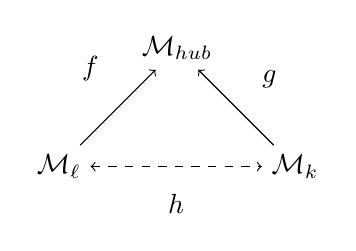
\begin{tikzpicture}
\node (M1) at (0,0) {$\mathcal{M}_\ell$};
\node (M2) at (3,0) {$\mathcal{M}_k$};
\node (Mhub) at (1.5,1.5) {$\mathcal{M}_{hub}$};
\draw[->] (M1) -- node[label={[label distance=0.1cm]120:$f$}] {} (Mhub);
\draw[->] (M2) -- node[label={[label distance=0.1cm]30:$g$}] {} (Mhub);
\draw[<->,dashed] (M1) -- node[label={[label distance=0.1cm]270:$h$}] {} (M2);
\end{tikzpicture}
\end{center}

There are several possiblities on how to find the map
$h$. Without loss of generality, we assume that
$h:\mathcal{M}_\ell \rightarrow \mathcal{M}_k$. Let
$\hat{f},\hat{g}$ and $\hat{h}$ denote the point-to-point
correspondences between the respective spaces. Note that this
implies that $h$ should be an extension of $\hat{h}$ (likewise
for $f$ and $g$).

In the following section we outline some methods for computing
$h$ using information  about $f$ and $g$.
\end{comment}
\begin{comment}
\section{APPROACHES
The most straightforward approach is to augment $\hat{h}$ with
relevant correspondences in $\hat{f}$ and $\hat{g}$. That is we
can define the new set of correspondences by
\begin{equation}
\hat{h} \coprod  (\hat{g}^{-1}\cdot \hat{f})
\end{equation}
Note that $\hat{g}^{-1}$ is not a true inverse but rather is
defined on as the co-image of $\hat{g}$.  That is, the disjoint
union of the initial set of correspondences augments with the
correspondences which can be composed through the hub
language. This implies that we only use part of the hub language,
namely $(\im \hat{f} \cap \im \hat{g})$. This requires all the
correspondences to be consistent (that the above diagram
commutes), which in the case of Wikipedia they are. It remains an
interesting open problem how to deal with inconsistencies.

An alternative approach is to learn $f$ and $g$ independently and
as above compose the linear maps. Therefore define $h = g^{-1}
\cdot f$. Since the maps are generally full rank, it can be
assumed that the inverse exists. Note that in this approach,
composition is simply multiplication (due to the linearity of the
operators).

Anything else?
\end{comment}

%Pairwise retrieval all
\begin{table*}[htbp]
\begin{center}
\caption{CL-LSI MAPR retrieval in common semantic space}
\label{lsi_common}
\begin{tabular}{|c|c|c|c|}\hline
&{\bf sl}& {\bf en}   & {\bf hi}\\\hline
{\bf sl} &0 & 0.77 & {\bf 0.45}\\\hline
{\bf en} &0.73 & 0 & 0.64\\\hline
{\bf hi} & {\bf 0.38} & 0.67 & 0\\\hline
\end{tabular}
\hspace{0.5cm}
\begin{tabular}{|c|c|c|c|}\hline &{\bf sl}& {\bf en}   & {\bf hi}\\\hline{\bf sl} & 0 & 0.81 & {\bf 0.6}\\\hline {\bf en} & 0.77 & 0 & 0.71\\\hline {\bf hi} &{\bf 0.61} & 0.76 & 0 \\\hline\end{tabular}
\hspace{0.5cm}
\begin{tabular}{|c|c|c|c|}\hline&{\bf sl}& {\bf en}   & {\bf hi}\\\hline {\bf sl} & 0 & 0.37 & {\bf 0.22}\\\hline {\bf en} & 0.49 & 0 & 0.36\\\hline {\bf hi} & {\bf 0.11} & 0.29 & 0 \\\hline\end{tabular}\\
\vspace{0.1cm}
\hspace{1cm}All \hspace{3.7cm} Common\hspace{3.7cm} Empty \hspace{0.7cm} \ \\
\end{center}
\end{table*}
%Retrieval using the whole information available
%All
\vspace{-0.2cm}
\section{EXPERIMENTS}
\vspace{-0.2cm}

Experiments were performed using an alignment obtained by
Wikipedia on several languages. Specifically we used Slovenian
(sl, 91272 words), English (en, 344517 words) and Hindi (hi,
72063 words). The markup in brackets denotes language and number
of words in each dictionary.  As a preprocessing step, all stub
documents with fewer than $20$ different words were dropped to
improve the quality of the data.  The remaining alignment
consists of $44426$ Slovenian-English correspondences, $4034$
Slovenian-Hindi correspondences, $14121$ English-Hindi
correspondences and $4017$ joint Slovenian-English-Hindi
correspondences.  After stub removal we keep $614$ of the initial
$1000$ test documents and remove them from the training data.


Retrieval can be done in five essentially different ways using
our metric space approach:
\begin{enumerate}
\item $sl\mapsto {\bf hi},$
\item $hi\mapsto {\bf sl}.$
\item $sl\mapsto {\bf en = hub = en} \mapsfrom
hi,$
\item $sl\mapsto
en \mapsto {\bf hi}$
\item $hi\mapsto en \mapsto {\bf sl}.$
\end{enumerate}
Bold denotes the space where retrieval is done. The first two
represent a direct mapping $sl \leftrightarrow hi$, while the
remaining methods map to a common hub space (in this case
English), with retrieval occurring either in the target language
or the hub language.

To see the amount of information present in the hub languages, we
performed tests on three substantially different datasets
\begin{itemize}
\item \emph{all} -- we use all alignment information available,
\item \emph{common} -- we use only alignment information consistent
through all three languages
\item  \emph{empty} -- we remove all common
alignment to simulate the case where we are forced to use hubs.
\end{itemize}

The evaluation criteria we use is the \emph{mean average
  precision mate retrieval score} (MAPR). This enables us to
compute a similarity between the documents and their translations
in the common vector space induced by the latent model or mapping
in the common space. Good models will map documents close to their
translations -- this indicates that some language independent
(semantic) information was captured.

Let the individual language we are considering be denoted by
$L_1$ and $L_2$.  Each (latent) model is given by projection
operators $P_1$ and $P_2,$ where one can be identity. We evaluate
each model by considering a pair of aligned test sets $X$ and
$Y$ in $L_1$ and $L_2$.
%
We select a query document $x \in X$ and denote the
corresponding translated document $y\in Y$.  We then compute
the projections $P_1 x$ and $P_2 Y$ and rank the elements of
$P_2 Y$ by their similarity to $P_1 x$ in the projection
space (measured by cosine similarity). The mean average precision
mate retrieval score is the inverse of the rank of $P_2 y$. If
only one score is displayed, then this is the average of the
inverse of the rank of $P_1 x$ and the inverse of the rank of
$P_2 y$.
\vspace{-0.2cm}
\subsection{Methods used}
\vspace{-0.2cm}
\begin{table*}[!htbp]
\begin{center}
\caption{\label{lsi_all}CL-LSI MAPR retrieval, full pairwise space}
\begin{tabular}{|c|c|c|c|}\hline & sl & en & hi\\\hline sl & 0 & 0.82 & {\bf 0.57}\\\hline en & 0.77 & 0 & 0.73\\\hline hi & {\bf 0.6} & 0.78 & 0\\\hline\end{tabular}
%Common
\hspace{0.75cm}
\begin{tabular}{|c|c|c|c|} \hline& sl & en & hi \\\hline sl & 0 & 0.81 & {\bf 0.58}\\\hline en & 0.77 & 0 & 0.71\\\hline hi & {\bf 0.58} & 0.77 & 0\\\hline\end{tabular}
%Empty
\hspace{0.75cm}
\begin{tabular}{|c|c|c|c|}\hline & sl & en & hi \\\hline sl & 0 & 0.78 & 0\\\hline en & 0.7 & 0 & 0.71\\\hline hi & 0 & 0.77 & 0 \\\hline\end{tabular}\\
\vspace{0.1cm}
\hspace{1cm}All \hspace{3.7cm} Common\hspace{3.7cm} Empty \hspace{0.7cm} \ \\
\end{center}
\end{table*}

In addition to studying the difference in performance depending
on which space we perform the retrieval in, there is also the
question of how we find the maps.

One approach is to learn the map from the aligned sets $X$ and
$Y$ to use a least squares low rank approach.  That is, we find W
of rank $k$ with which minimizes $\min || W X - Y||_F$ where $k$
is an input parameter. The solution can be obtained using a
truncated SVD of the input $X,$ $W = Y X^+,$ $X = U \Sigma V^*,$
$X_k^+ = V_k \Sigma_k^{-1} U_k,$ where $+$ denotes the pseudo
inverse of matrix $X.$ To speed up the computation, a low rank
approximation of matrix $Y$ is used.  We always use truncated
SVDs of size $1000.$ This approach is denoted as LSQ.

Another method that can be used to relate two aligned sets is
regression canonical correlation analysis (RCCA) that is
described in \cite{ccar}.  Essentially, this results
in the map $q \mapsto (XX')^{-1} X Y' q \approx U_k \Sigma_k^{-1}
V_k^* Y' q$. Note that this must be used on (implicitly) centered
data. Centering explicitly however, is not feasible due to the
large number of words which would result in prohibative RAM
requirements.  Again we use low rank approximations of implicitly
centered $Y$'s to reduce the time complexity and space
complexity.

The third method we use is CL-LSI, latent semantic indexing. It
is described in \cite{cl-lsi}.  This method enables us to compare
documents in the common semantic space.  For the sake of clarity,
we described this method only for two or three aligned document
sets $X_1, X_2, X_3.$ First, we do the SVD decomposition of the
glued aligned documents, then we decouple the basis and map in
the common subspace.
\[
\begin{bmatrix}
X_1\\
X_2
\end{bmatrix} =
\begin{bmatrix}
U_1\\
U_2
\end{bmatrix} \Sigma V^*, \quad
\begin{bmatrix}
X_1\\
Y_1\\
Z_1
\end{bmatrix} =
\begin{bmatrix}
U_1\\
U_2\\
U_3\\
\end{bmatrix} \Sigma V^*,
\]
The map to the common semantic space can be described as $x_i
\mapsto V \Sigma^+ U_i^+ x_i$ for $i=1, 2, 3,$ where we overload
symbols $\Sigma$ and $V$.

To map to English (hub) using the full alignment, we first map
Slovenian $x_1$ to the English word space as $x_1 \mapsto
U^{12}_2 (U^{12}_1)^+ x_1$ and Hindi $x_3$ to English word space
as $x_3 \mapsto U^{23}_1 (U^{23}_2)^+ x_3$. This can be done
efficiently.  Similary we map Slovenian $x_1$ to the
Hindi-English semantic space through English as $x_1 \mapsto
U^{12}_2 (U^{12}_1)^+ x_1 = y_1 \mapsto (U^{23}_1)^+ y_1$ and
Hindi $x_3$ to Hindi-English semantic space $x_3 \mapsto
(U^{23}_2)^+ x_3.$

Mapping through the hub in CL-LSI case enables us to compare
documents in the semantic space which as we will see seems to
boost performance.  In the \emph{all} and
\emph{empty} datasets. we glue documents together all three
languages despite the lack of an alignment to see how performance
degrades in comparison with using the hub.

%Opiši MAPR in povdari, da preslikave z regresijo in LSQ niso simetrične.
%Komentiraj rezultate.
%Zaključek hub lahko izkoristimo, vendar so potrebne še nadaljnje raziskave.
\vspace{-0.2cm}
\subsection{Results}
\vspace{-0.2cm}
As expected, the retrieval is dependent on the mapping used.  It
is important to note the lack of symmetry in retrieval for the
computed RCCA and LSQ mappings.  This is to be expected as we
only use the information about the target(or alternatively the
source) and no common information (as covariance). To illustrate
this, RCCA mapping on the \emph{all} dataset, $hi \mapsto {\bf
  sl},$ results in a retrieval score of $0.55$, but RCCA mapping
other way around on the same dataset, $sl \mapsto {\bf hi},$
results in a retrieval score of $0.45$.

Better performance could be obtained by using canonical
correlation analysis (CCA) although this is a more difficult
computationally and has not yet been tested.  A similar (dual) situation
holds for LSQ mapping where we use only the information about the
source space (rather than the target space).


From Table \ref{regress_lsq} it is not immediately clear which
option of using the hub is the best.  Using the hub does not
improve performance even if we use the whole alignment
information available.  But is clearly the only option if there
is no alignment information through all languages or this
alignment is too small.

The CL-LSI method behaves more consistently and outperforms other
methods.  In this case, the better option is to go through the
hub as we can then compare documents in the semantic space at the
end.  Further tests are needed to better understand this behavior.

In Tables \ref{lsi_common} and \ref{lsi_all} we additionally
display retrieval using mapping in the common semantic space and
using full pairwise alignment, respectively. This gives us an idea
about the quality of each mapping.


\vspace{-0.2cm}
\subsection{Ideal retrieval under  misalignment}
\vspace{-0.2cm}
Consider the \emph{empty} scenario described above: we wish to
compare documents between languages $L_1$ and $L_2$, but we only
have aligned sets for the two languages with a third language
$L_{\mathrm{hub}}$. Our aligned sets $T_1$ and $T_2$
correspond to $ L_1\mapsto L_{\mathrm{hub}}$ and $ L_2\mapsto
L_{\mathrm{hub}}$ respectively.

%: $(A_h, H_a)$ and $b$ and
%language $h$: $(B_h, H_b)$, where $H_A \cap H_B = \emptyset$ (no
%document is shared), where



%$A_h \in \mathbb{R}^{f_a \times
%  n_{a\cap b}}, H_a \in \mathbb{R}^{f_h \times n_{a\cap h}}, H_b
%\in \mathbb{R}^{f_h \times n_{b\cap h}}, B_h \in \mathbb{R}^{f_b
%  \times n_{b\cap h}}$.
We assume that no document is shared between $T_1$ and
$T_2$. Since the alignments are disjoint it may follow that
$rank( T_1 \oplus T_2) = rank( T_1) + rank( T_2)$.
In such cases no nonzero document can be exactly
represented in both bases.
%
%
Let $f_{1}: L_1 \rightarrow L_{\mathrm{hub}}$ and $f_{2}: L_2
\rightarrow L_{\mathrm{hub}}$ represent the regression maps
constructed using the alignment. By using the maps we can cast
the information retrieval problem between documents in languages
$L_1$ and $L_2$ as a monolingual information retrieval problem
$L_{\mathrm{hub}}$. Since $im(f_{1}) \subset span(T_1)$ and
$im(f_{2}) \subset span(T_2)$, all inter-lingual similarities
will be reduced due to the mis-alignment of the spaces
$span(T_1)$ and $span(T_2)$ (rather than all of
$L_{\mathrm{hub}}$). Since the quality of retrieval typically
degrades when no direct alignments are available(see Section
4.2), we investigate what is the best possible retrieval under
the mis-aligned spaces. That is, what is the highest possible
retrieval score on the test set, provided that the images of
$f_{1}, f_{2}$ are restricted to $span(T_1)$ and $span(T_2)$
respectively.
%
As in the previous section, the experiment is based on IR between
Wikipedia pages written in Slovenian ($sl$), Hindi($hi$) and English
($en$). The English language represents the hub language with the
following document matrices: $T_1 \in \mathbb{R}^{406,044
  \times 41,529}, T_2 \in \mathbb{R}^{406,044 \times
  10,331}$, and ${T}_{\mathrm{test}} \in \mathbb{R}^{406,044 \times
  604}$.

$T_{\mathrm{test}}$ is aligned to $A_{\mathrm{test}}$ and $B_{\mathrm{test}}$ and
  $rank([T_1 T_2]) = rank(T_1) + rank(T_2)$. In the ideal case
  $A_{\mathrm{test}}$ and $B_{\mathrm{test}}$ would be mapped to $T_{\mathrm{test}}$ under
  $f_{1}$ and $f_{2}$.

 Let $P_X(\cdot)$ denote the orthogonal projection map to the
 column space of the matrix $X$. Since the images of $f_{1}$ and
 $f_{2}$ are spanned by $T_1$ and $T_2$, the test sets would
 ideally be mapped to $P_{T_1}(T_{\mathrm{test}})$ (ideally
 projected Slovene test documents) and
 $P_{T_2}(T_{\mathrm{test}})$ (ideally projected Hindi test
 documents).


The mean average precision mate retrieval scores we obtain are:
$0.995$ when $A_{test} = \text{query}$, $B_{test} =
\text{target}$ and $0.969$ when $A_{test} = \text{target}$,
$B_{test} = \text{query}$. High retrieval scores indicate that
the space of possible maps admits good quality solutions. This
result shows potential for improving the retrieval quality.
\vspace{-0.2cm}
\section{CONCLUSION}
\vspace{-0.2cm}
The experiments we ran serve two main purposes: the first is an
investigation of the performance of using a hub language to
enable us to compare languages where alignments may not exist
using various different maps and approaches to learning the
maps. The second is a structural study, which illustrates how
much information is present in the maps. In principle this second
part, illustrates that it is possible to find a
linear representation in the hub space which yields very high
retrieval score, even with no overlap in the alignment. This
means that it should be possible to learn maps with very high
retrieval rates.

The first set of experiments show that with the approprate
preprocessing, going throuh hub languages work reasonably
well. However, the lack of symmetry (whereas correspondences are
symmetric) in the maps suggests that this may be degrading
performance. A method which takes both structures into
account may perform better at a higher computational
cost. Further, with no alignment there are distribution issues
which must be addressed (each language has a different
distribution of documents in its monolingual metric space),
suggesting that techniques based on transport distance may prove
effective.
\vspace{-0.2cm}
\section{ACKNOWLEDGEMENTS}
\vspace{-0.2cm}
The authors gratefully acknowledge that the funding for this work was provided by the projects X-LIKE (ICT-257790-STREP), PlanetData (ICT-257641-NoE) and META-NET (ICT-249119-NoE).

\ \\
 \textbf{\large References} \vspace*{1.3ex} \newcounter{mycount} \begin{list}{[\arabic{mycount}]}
  {\usecounter{mycount}\setlength{\leftmargin}{0.5cm}
   \setlength{\parsep}{0pt}\setlength{\itemsep}{2pt}
   \setlength{\labelsep}{0.1cm}}


\bibitem{cl-lsi}
S.~T. Dumais, T.~A. Letsche, M.~L. Littman, and T.~K. Landauer.
\newblock Automatic cross-language retrieval using latent semantic indexing.
\newblock In {\em AAAI'97 Spring Symposium Series: CrossLanguage Text and
  Speech Retrieval}, pages 18--224, 1997.

\bibitem{iti}
Primoz~\v Skraba, Jan~Rupnik, Andrej~Muhi\v c.
\newblock Cross-Lingual Document Similarity.
\newblock In {\em ITI 2012 Information Technology Interfaces}.

\bibitem{ccar}
Jan~Rupnik, Bla\v z Fortuna.
\newblock Regression Canonical Correlation Analysis.
\newblock Learning from Multiple Sources, NIPS Workshop, 13 Dec 2008 Whistler Canada.

\bibitem{nips}
Primoz~\v Skraba, Jan~Rupnik, Andrej~Muhi\v c.
\newblock Low-rank approximations for large, multi-lingual data.
\newblock NIPS Workshop on Low Rank Approximation and Sparse Representation, 2011.
\end{list}

\end{document}
